\documentclass[11pt, a4paper]{article}
%\usepackage{proj1}
\usepackage{natbib}
\usepackage{fancyhdr}  
\usepackage{subcaption}
\usepackage{caption}
\usepackage{graphicx}
\usepackage{numprint}
\usepackage{multirow}
\linespread{1.25} 
\setlength{\parindent}{0cm}
\graphicspath{{Images/}}
\usepackage{hyperref}
\usepackage{amsmath}
\usepackage{amsfonts}
\usepackage{amssymb}
\usepackage{amsthm}
\usepackage{mathtools}
\usepackage{commath}
\usepackage{bbm}

%\usepackage[sc,osf]{mathpazo}
\usepackage{subcaption}
\usepackage[a4paper, top=1in, left=1.0in, right=1.0in, bottom=1in, includehead, includefoot]{geometry} %Usually have top as 1in

\usepackage{listings}
\usepackage{color} %red, green, blue, yellow, cyan, magenta, black, white
\definecolor{mygreen}{RGB}{28,172,0} % color values Red, Green, Blue
\definecolor{mylilas}{RGB}{170,55,241}


\hypersetup{colorlinks,linkcolor={black},citecolor={blue},urlcolor={black}}
\usepackage{color}
\urlstyle{same}


\theoremstyle{definition}
\newtheorem{definition}{Definition}[section]

%\newcommand{\Sta}{\rho}
\newcommand{\adja}{q_a}
\newcommand{\adjb}{q_b}
\newcommand{\adjaB}{q_{a,\partial \Omega}}
\newcommand{\adjbB}{q_{b,\partial \Omega}}
%\newcommand{\Con}{u}
\newcommand{\ra}{\rho_a}
\newcommand{\rb}{\rho_b}
\newcommand{\w}{\mathbf{w}}
\newcommand{\Stav}{\mathbf{v}}
\newcommand{\Adja}{\mathbf{p}}
\newcommand{\Adjb}{q}
\newcommand{\Adjc}{{p}_{\partial \Sigma}}
\newcommand{\Con}{\mathbf{f}}
\newcommand{\n}{\mathbf{n}}
\newcommand{\h}{\mathbf{h}}
\newcommand{\K}{\mathbf{K}}


\pagenumbering{gobble}
\begin{document}
	\section*{Problems solved using the MultiShape Code}
We consider the following optimal control problem:
\begin{align*}
&\mathcal{J}(\rho, \w) = \frac{1}{2}|| \rho - \widehat \rho||^2_{L_2(\Sigma)} + \frac{\beta}{2}|| \w ||^2_{L_2(\Sigma)}\\
&\text{subject to:}\\
&\frac{\partial \rho}{\partial t} = \nabla^2 \rho - \nabla (\rho \w) + \kappa \nabla \int_\Omega \rho(r) \rho(r') \K(r,r') dr'.
\end{align*}
\section{Example 1}
The initial configuration for this example is:
\begin{align*}
&\rho_0 = \exp(-2((y_1 - 0.5 )^2 + (y_2 + 0.5)^2))\\
&\w = \mathbf 0.
\end{align*}
The target $\widehat \rho$ is set by running a forward problem with the same $\rho_0$ but with constant velocity $\w = \mathbf{1}$.
The domain for this example is a quadrilateral and a wedge and can be seen in Figure \ref{Dom1}. The tolerances are $10^{-3}/ 10^{-7}$. Per shape $N = 20$ and $n = 20$. We plot the times $2/20$, $10/20$ and $19/20$.

\begin{figure}[h]
	\centering
	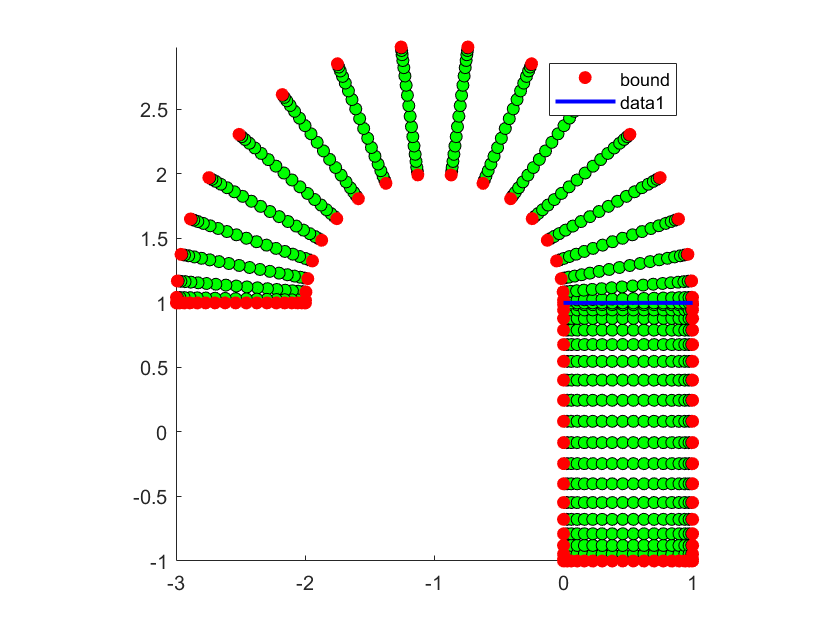
\includegraphics[scale=0.6]{Dom1.png}
	\caption{Domain Example 1} 
	\label{Dom1}
\end{figure}
Choosing $\kappa = -1$, we get $J_{FW} = 0.0251$, $J_{Opt} = 0.0020$. In Figure \ref{FEx1a}, $\widehat \rho$ and corresponding $\w$ are plotted, while in Figure \ref{FEx1b}, the optimal result is displayed. Choosing $\kappa = 1$, we get $J_{FW} = 0.0176$, $J_{Opt} = 0.0020$. In Figure \ref{FEx1c}, $\widehat \rho$ and corresponding $\w$ are plotted, while in Figure \ref{FEx1d}, the optimal result is displayed. It can be seen that while the attractive particles clump in the middle, the repulsive particles are clustered at the boundaries.
\begin{figure}[h]
	\centering
	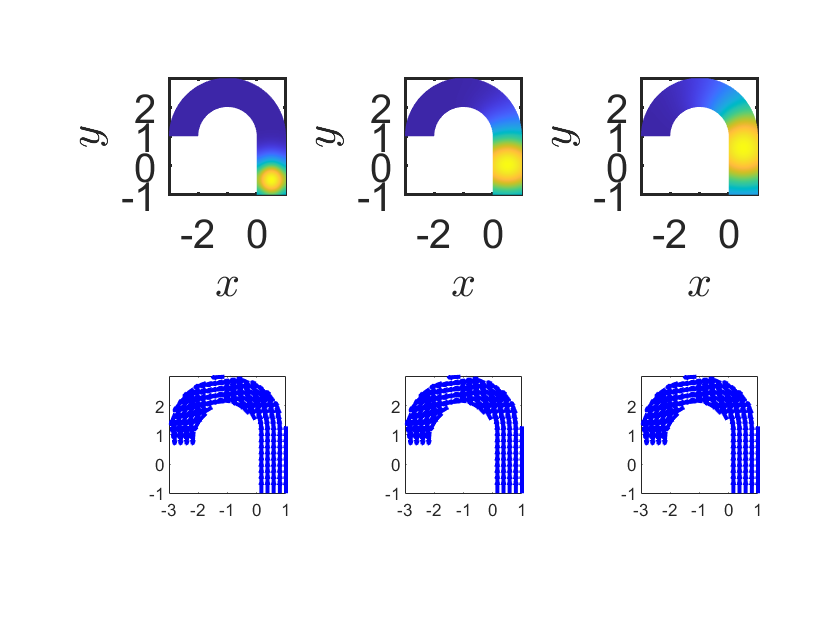
\includegraphics[scale=0.6]{FW1n1.png}
	\caption{Example 1, $\widehat \rho$, $\kappa = -1$} 
	\label{FEx1a}
\end{figure}
\begin{figure}[h]
	\centering
	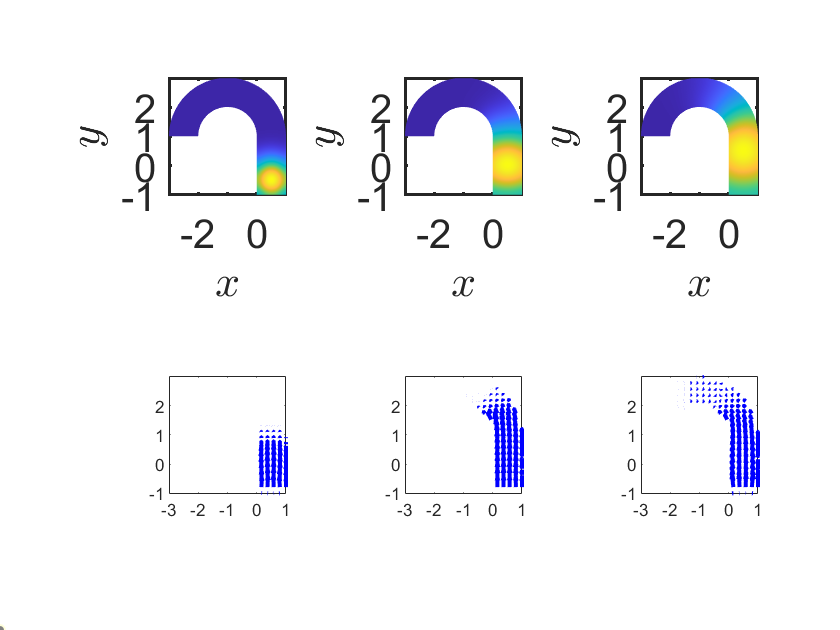
\includegraphics[scale=0.6]{Opt1n1.png}
	\caption{Example 1, optimal $\rho$ and $\w$, $\kappa = -1$} 
	\label{FEx1b}
\end{figure}

\begin{figure}[h]
	\centering
	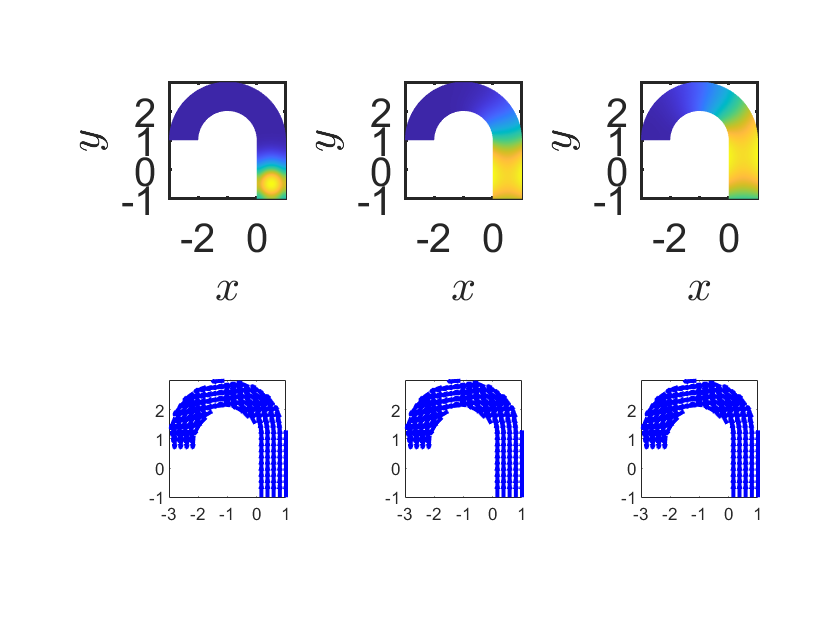
\includegraphics[scale=0.6]{FW11.png}
	\caption{Example 1, $\widehat \rho$, $\kappa = 1$} 
	\label{FEx1c}
\end{figure}
\begin{figure}[h]
	\centering
	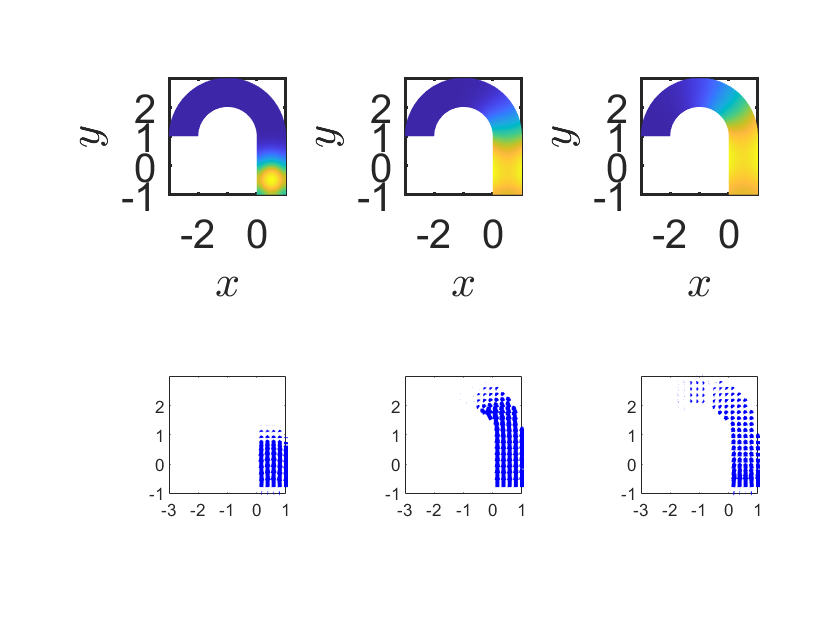
\includegraphics[scale=0.6]{Opt11.png}
	\caption{Example 1, optimal $\rho$, $\w$, $\kappa = 1$} 
	\label{FEx1d}
\end{figure}
(Note to self: this corresponds to Test10/ Example5a in code.)
\section{Example 2}
As initial configuration we choose:
\begin{align*}
&\rho_0 = \exp(-2((y_1 - 0.5 )^2 + (y_2 + 0.5)^2))\\
&\w = \mathbf{0}.
\end{align*}	
The target is a forward problem run with the same $\rho_0$ but with a constant background flow $\w = \mathbf{5}$. We run the problem up to time $2$, as opposed to time $1$ as usual. This is more stable than increasing the strength of the background flow. We still plot the time points $2/20$, $10/20$ and $19/20$. The domain of the problem is a channel, see Figure \ref{Dom2}.
\begin{figure}[h]
	\centering
	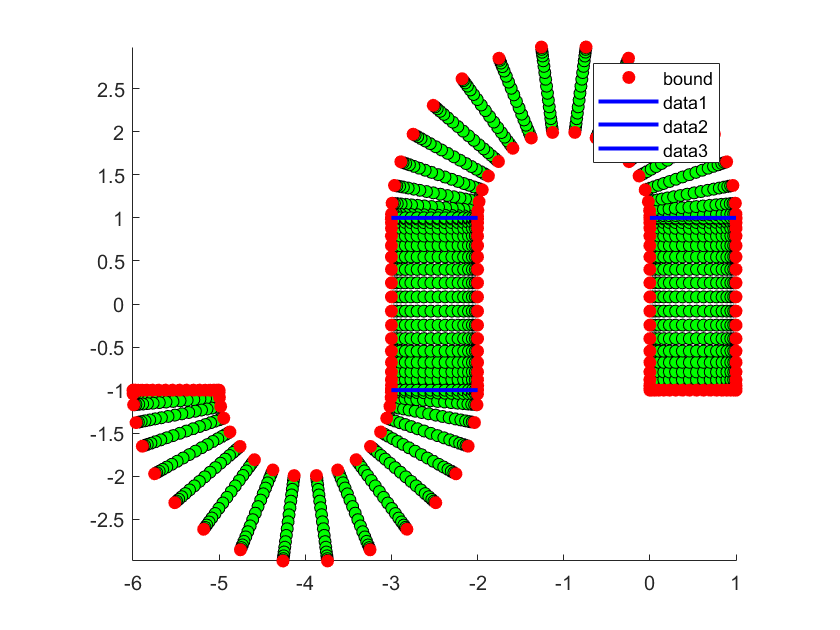
\includegraphics[scale=0.6]{Dom2.png}
	\caption{Domain Example 2} 
	\label{Dom2}
\end{figure}


Choosing $\kappa = -1$, we get $J_{FW} =  0.4111$, $J_{Opt} =  0.0807$. In Figure \ref{FEx2a}, $\widehat \rho$ and corresponding $\w$ are plotted, while in Figure \ref{FEx2b}, the optimal result is displayed. Choosing $\kappa = 1$, we get $J_{FW} =  0.3501$, $J_{Opt} =  0.0821$. In Figure \ref{FEx2c}, $\widehat \rho$ and corresponding $\w$ are plotted, while in Figure \ref{FEx2d}, the optimal result is displayed. Again, the difference between attractive and repulsive interaction is clearly displayed by the clustering of the particles in the channel. (Note to self: this is test 11a and Example4a) 
\begin{figure}[h]
	\centering
	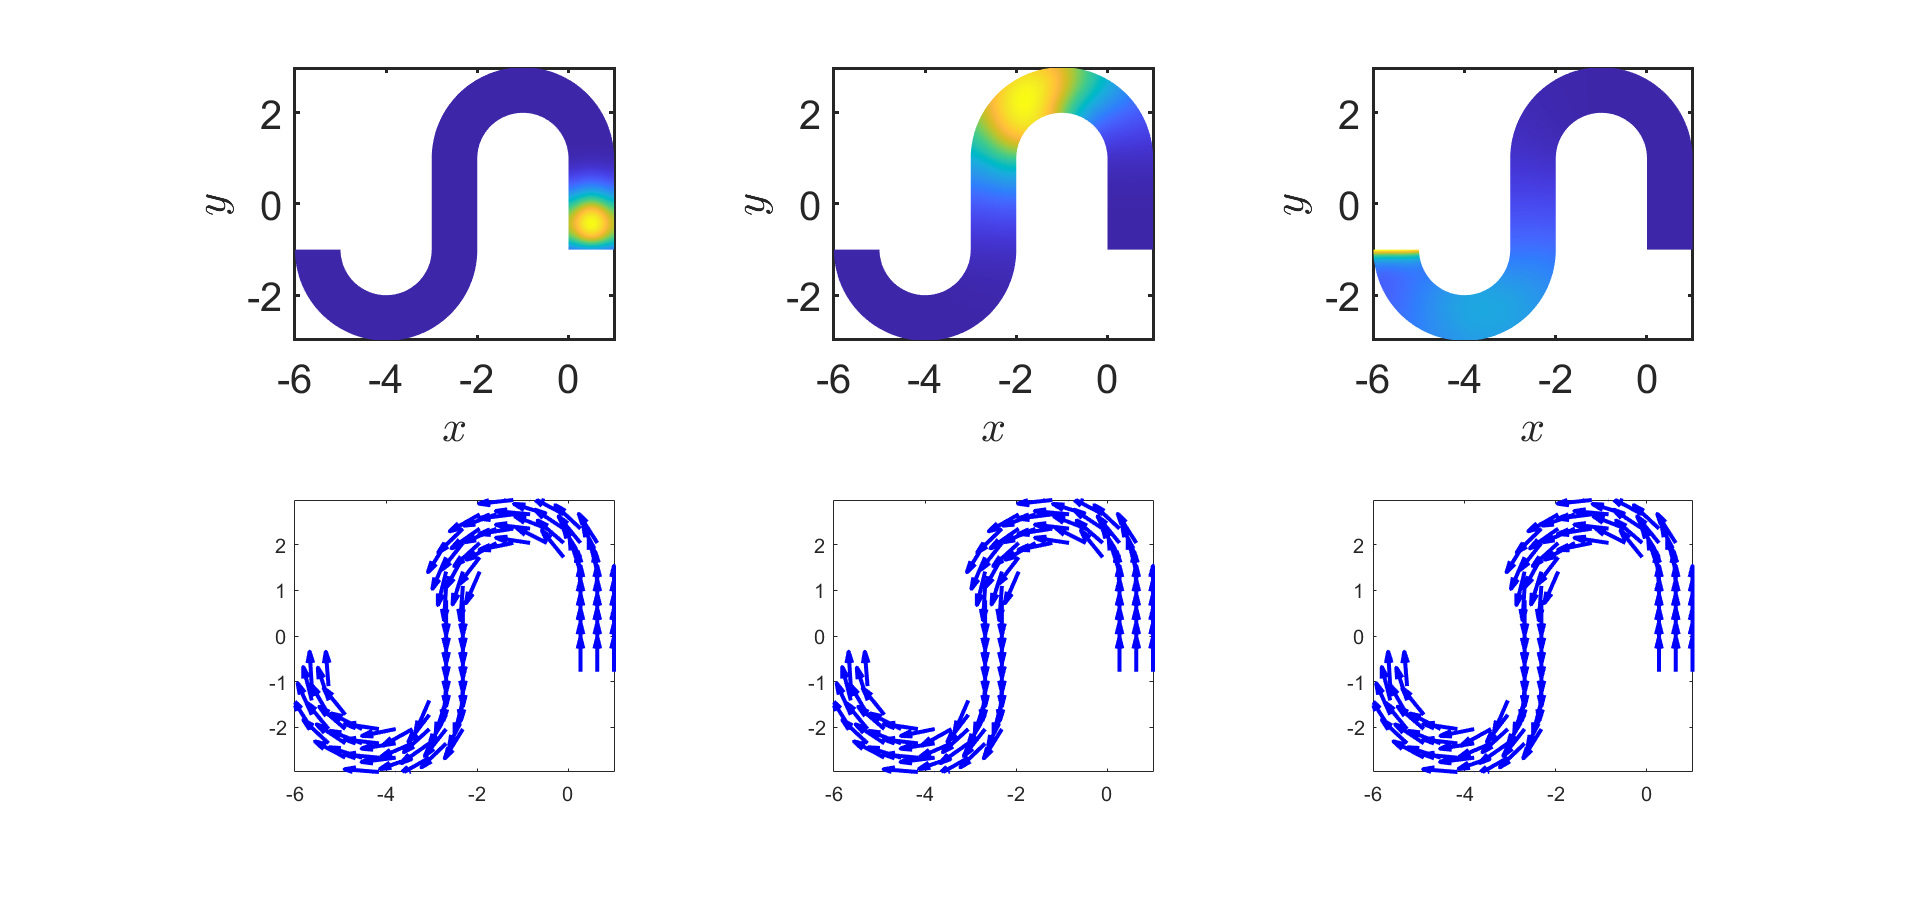
\includegraphics[scale=0.3]{FW2n1.png}
	\caption{Example 2, $\widehat \rho$, $\kappa = -1$} 
	\label{FEx2a}
\end{figure}
\begin{figure}[h]
	\centering
	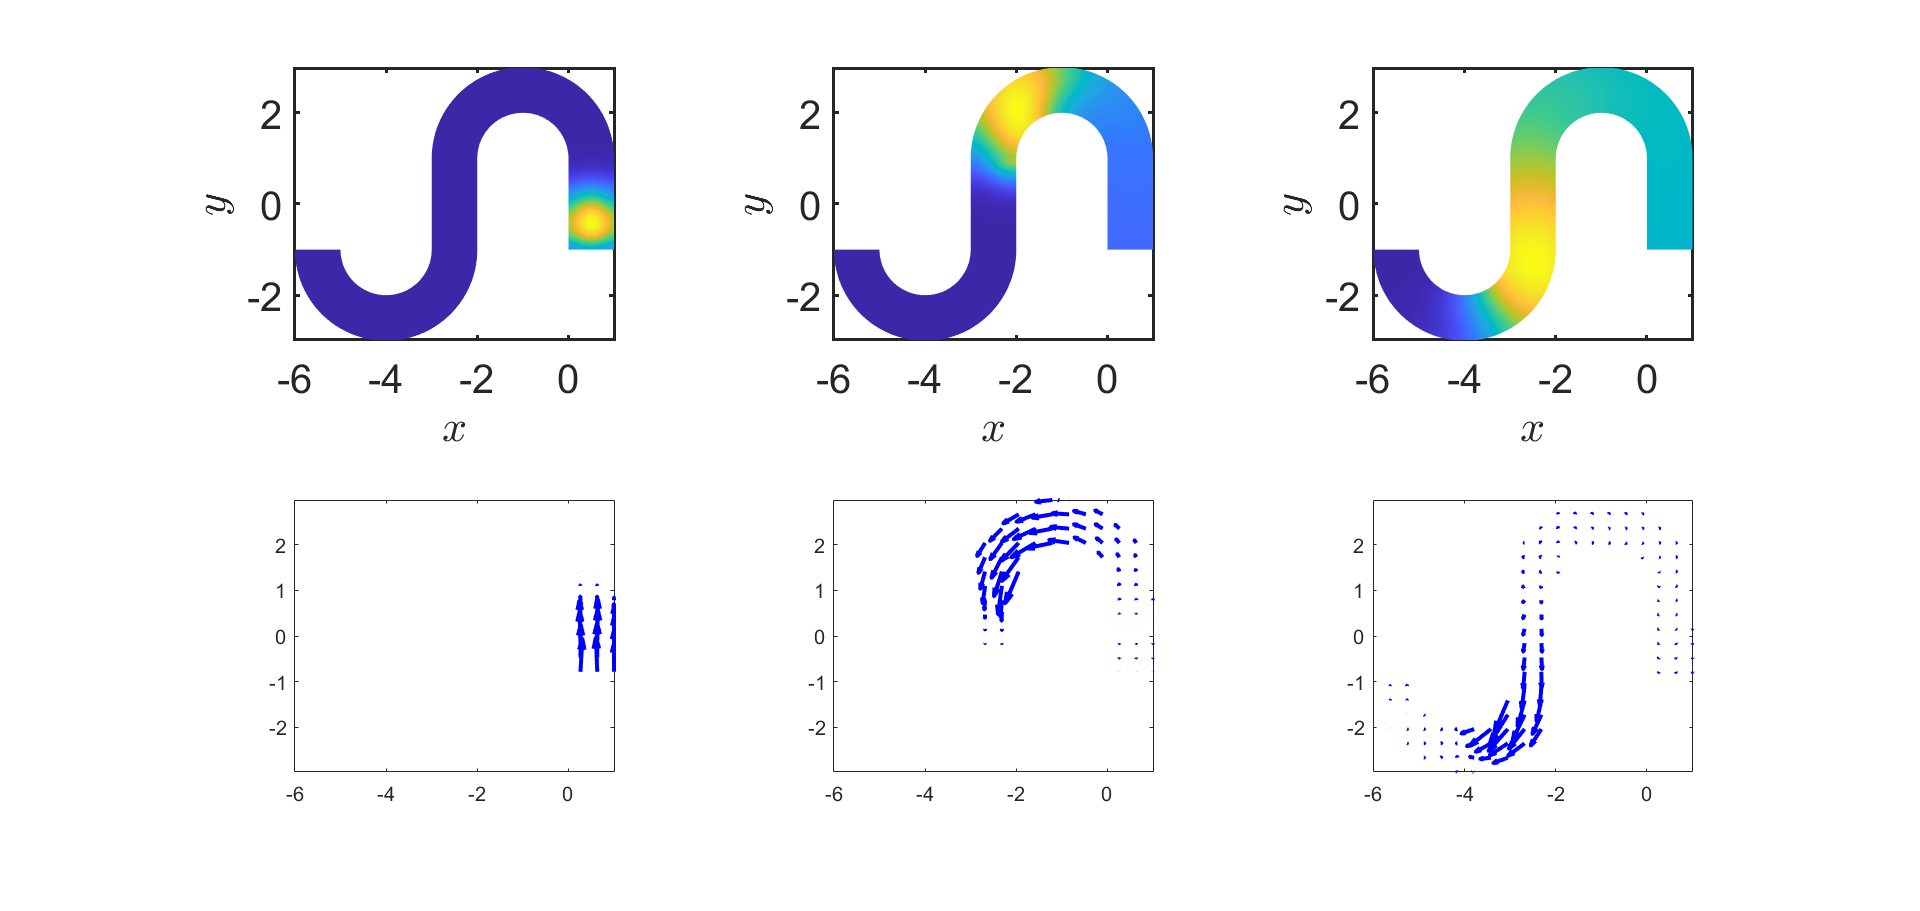
\includegraphics[scale=0.3]{Opt2n1.png}
	\caption{Example 2, optimal $\rho$ and $\w$, $\kappa = -1$} 
	\label{FEx2b}
\end{figure}

\begin{figure}[h]
	\centering
	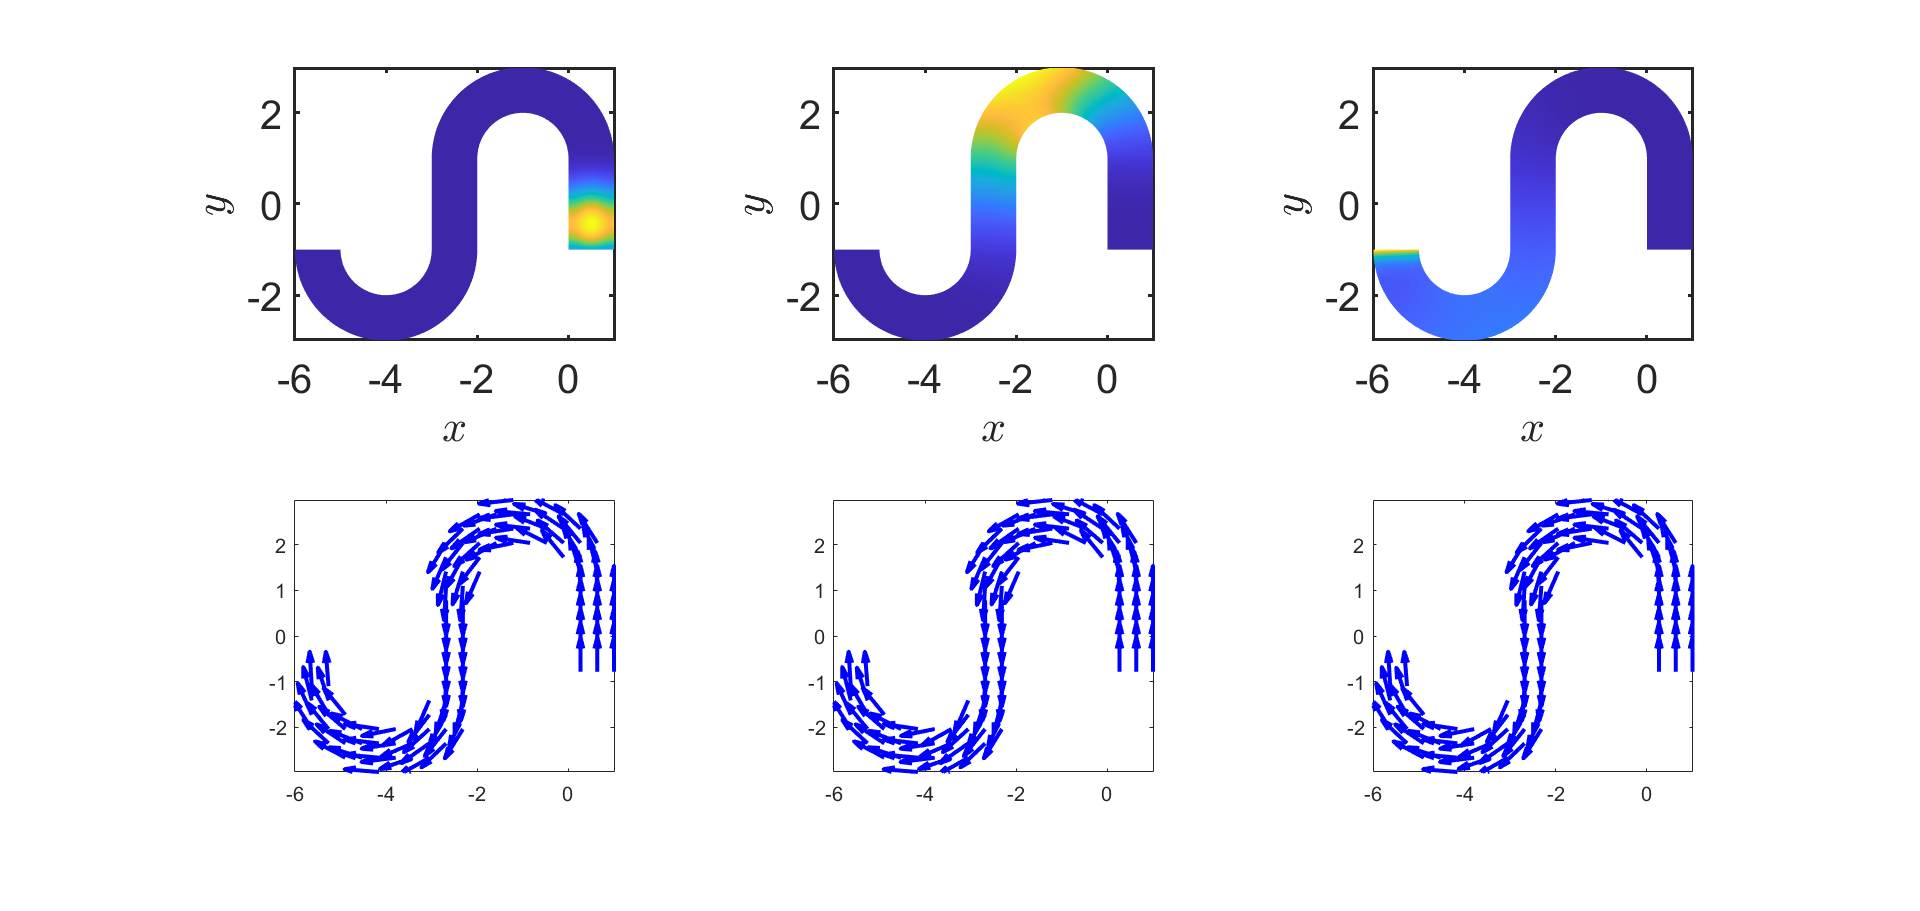
\includegraphics[scale=0.3]{FW21.png}
	\caption{Example 2, $\widehat \rho$, $\kappa = 1$} 
	\label{FEx2c}
\end{figure}
\begin{figure}[h]
	\centering
	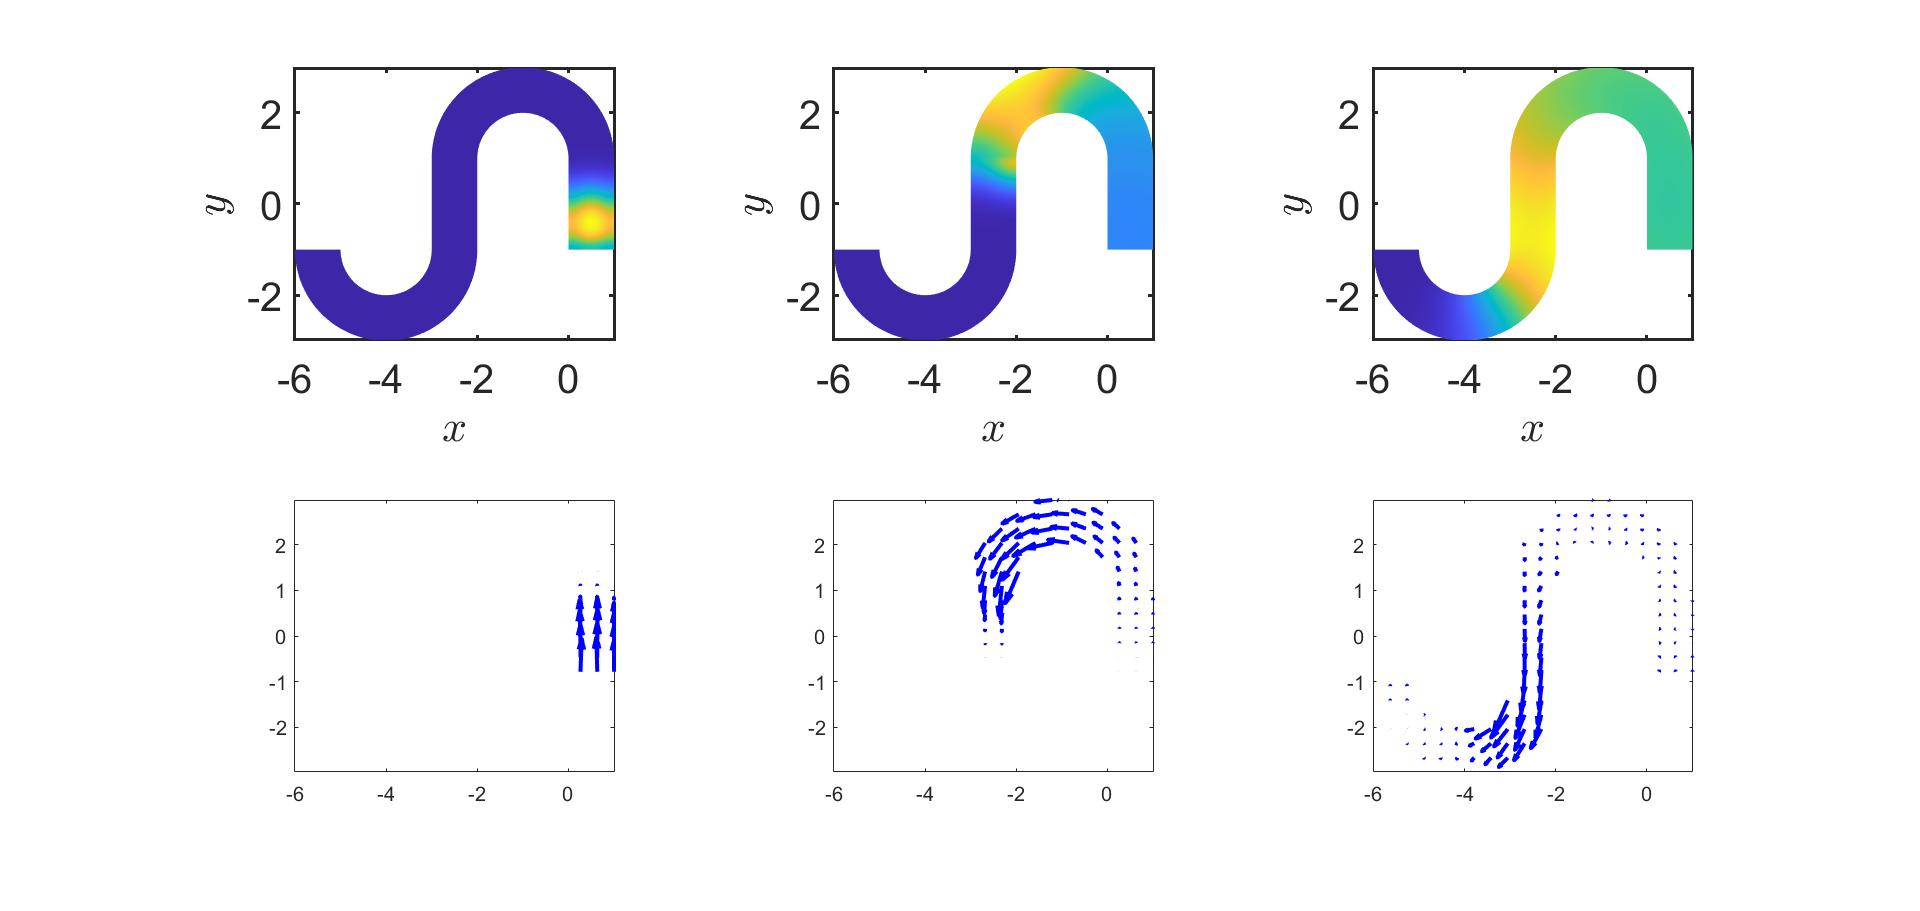
\includegraphics[scale=0.3]{Opt21.png}
	\caption{Example 2, optimal $\rho$ and $\w$, $\kappa = 1$} 
	\label{FEx2d}
\end{figure}







	
\section{Example 3}
As initial configuration we choose:
\begin{align*}
&\rho_0 = \exp(-2((y_1 + 1)^2 + (y_2 + 0.3)^2))\\
&\w = \mathbf{0}.
\end{align*}	
The target is a forward problem run with the same $\rho_0$ but with a background flow of constant one running along the domain. This and the domain of the problem can be seen in Figure \ref{Dom3}.
\begin{figure}[h]
	\centering
	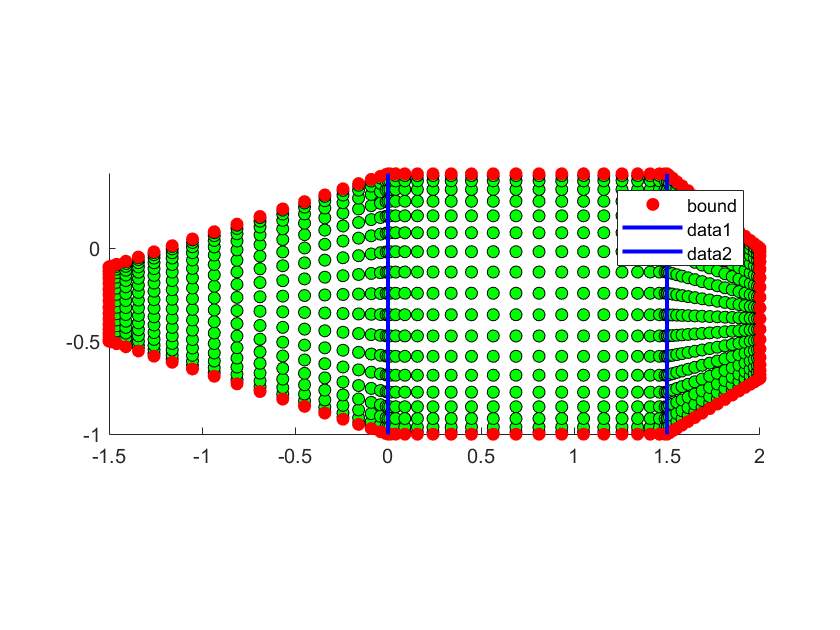
\includegraphics[scale=0.4]{Dom3.png}
	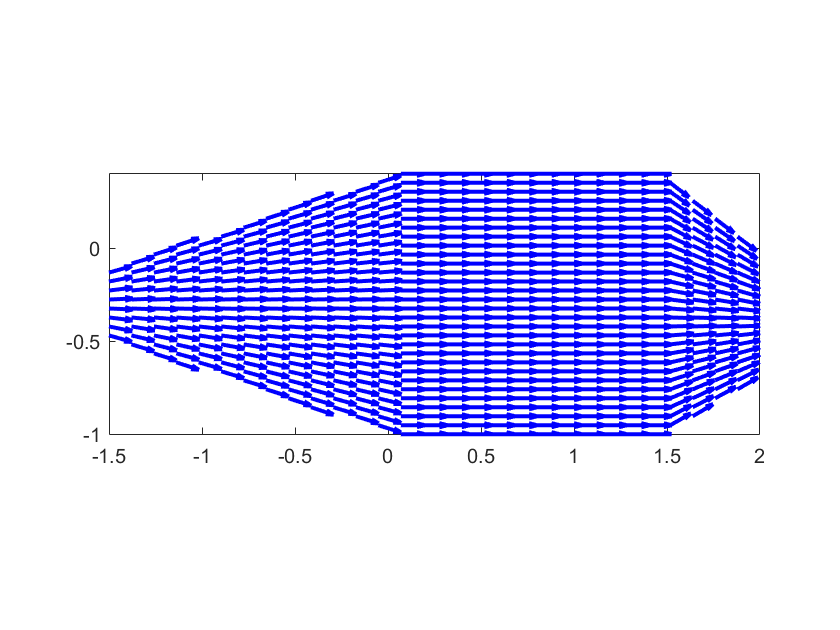
\includegraphics[scale=0.4]{Flow3.png}
	\caption{Domain and Flow Example 3} 
	\label{Dom3}
\end{figure}	
	
Choosing $\kappa = -1$, we get $J_{FW} = 0.0184$, $J_{Opt} = 9.5312 \times 10^{-4}$. In Figure \ref{FEx3a}, $\widehat \rho$ and corresponding $\w$ are plotted, while in Figure \ref{FEx3b}, the optimal result is displayed.
\begin{figure}[h]
	\centering
	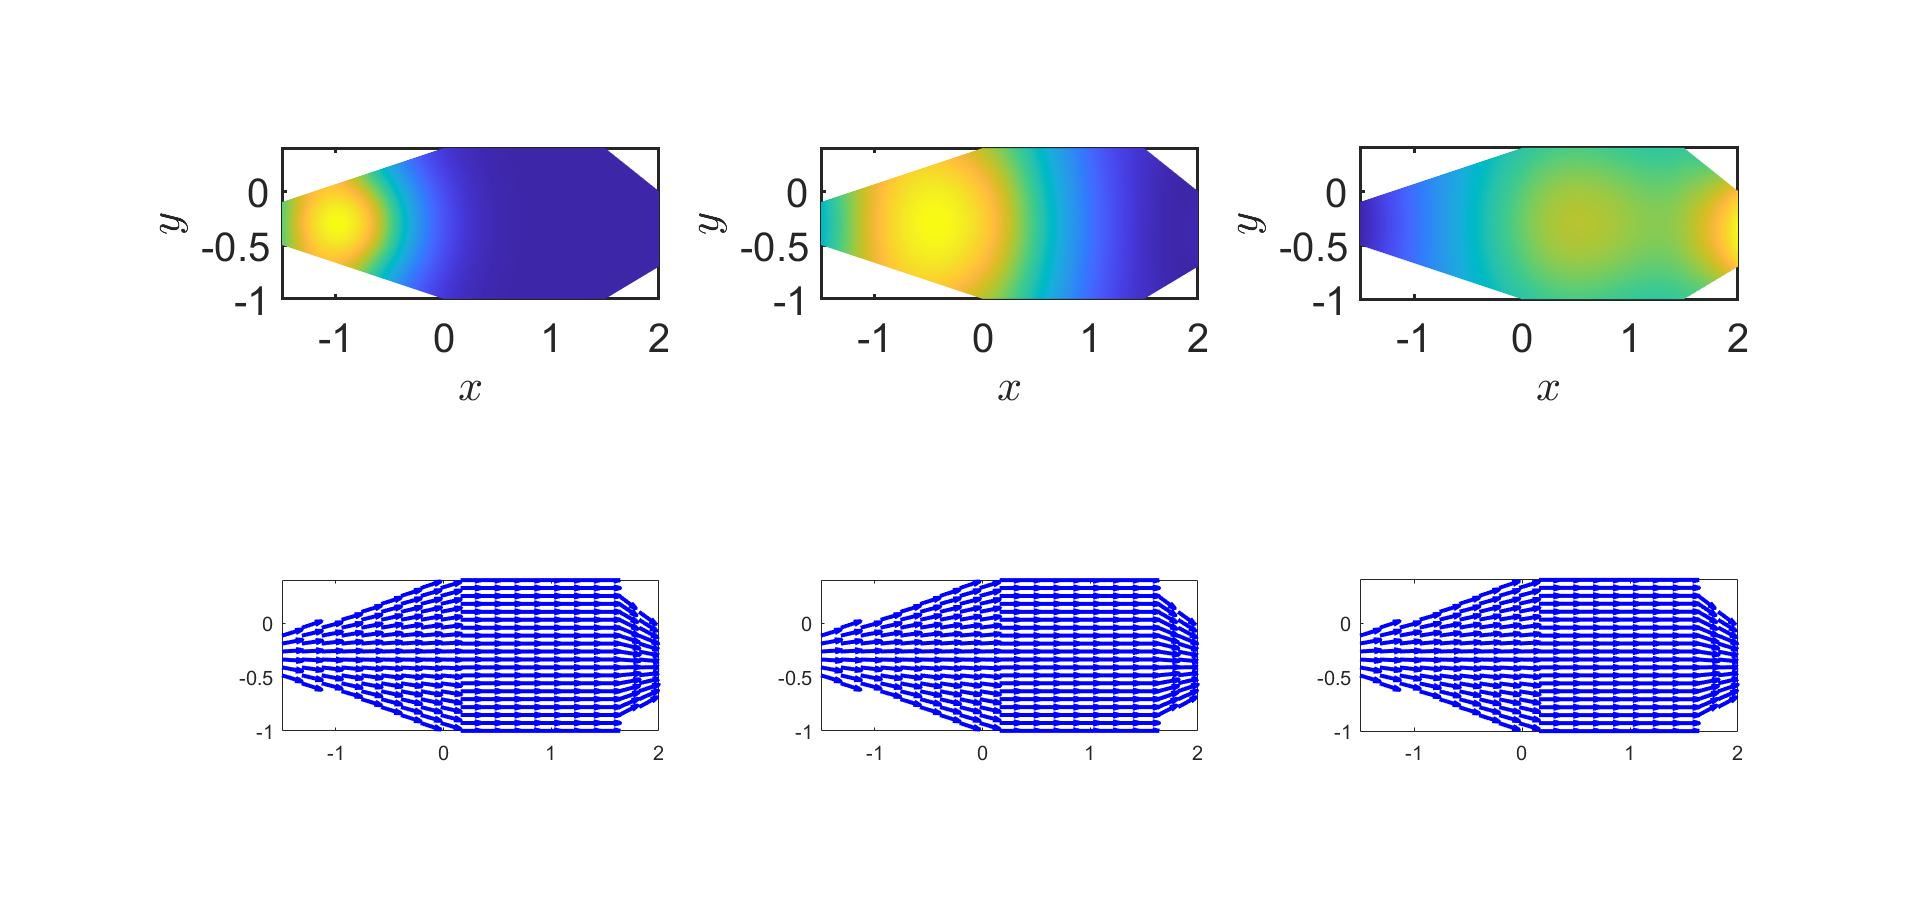
\includegraphics[scale=0.3]{FW3n1.png}
	\caption{Example 3, $\widehat \rho$, $\kappa = -1$} 
	\label{FEx3a}
\end{figure}
\begin{figure}[h]
	\centering
	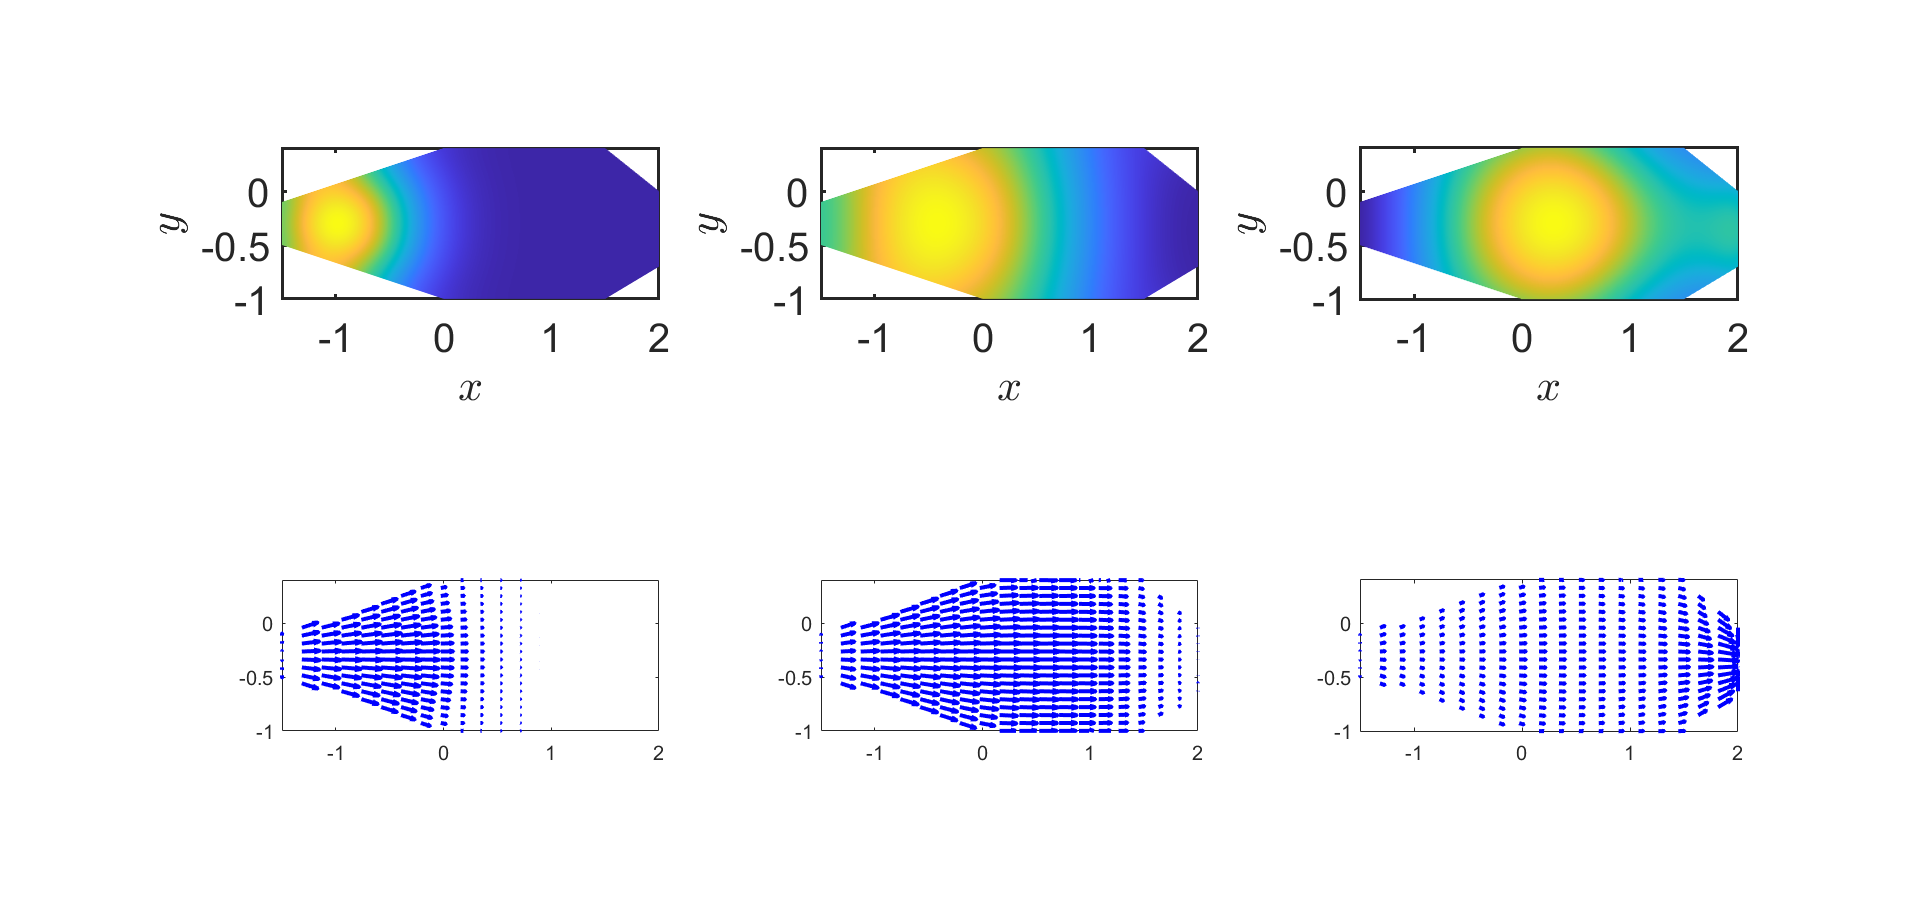
\includegraphics[scale=0.3]{Opt3n1.png}
	\caption{Example 3, optimal $\rho$ and $\w$, $\kappa = -1$} 
	\label{FEx3b}
\end{figure}	
	
Choosing $\kappa = 1$, we get $J_{FW} = 0.0150$, $J_{Opt} = 0.0010$. In Figure \ref{FEx3c}, $\widehat \rho$ and corresponding $\w$ are plotted, while in Figure \ref{FEx3d}, the optimal result is displayed. It is very obvious here how different the attractive and repulsive particles behave in this channel. It seems that the repulsive particles are clustering more on the sides and at the end of the channel, while the attractive particles are closer to the middle.
\begin{figure}[h]
	\centering
	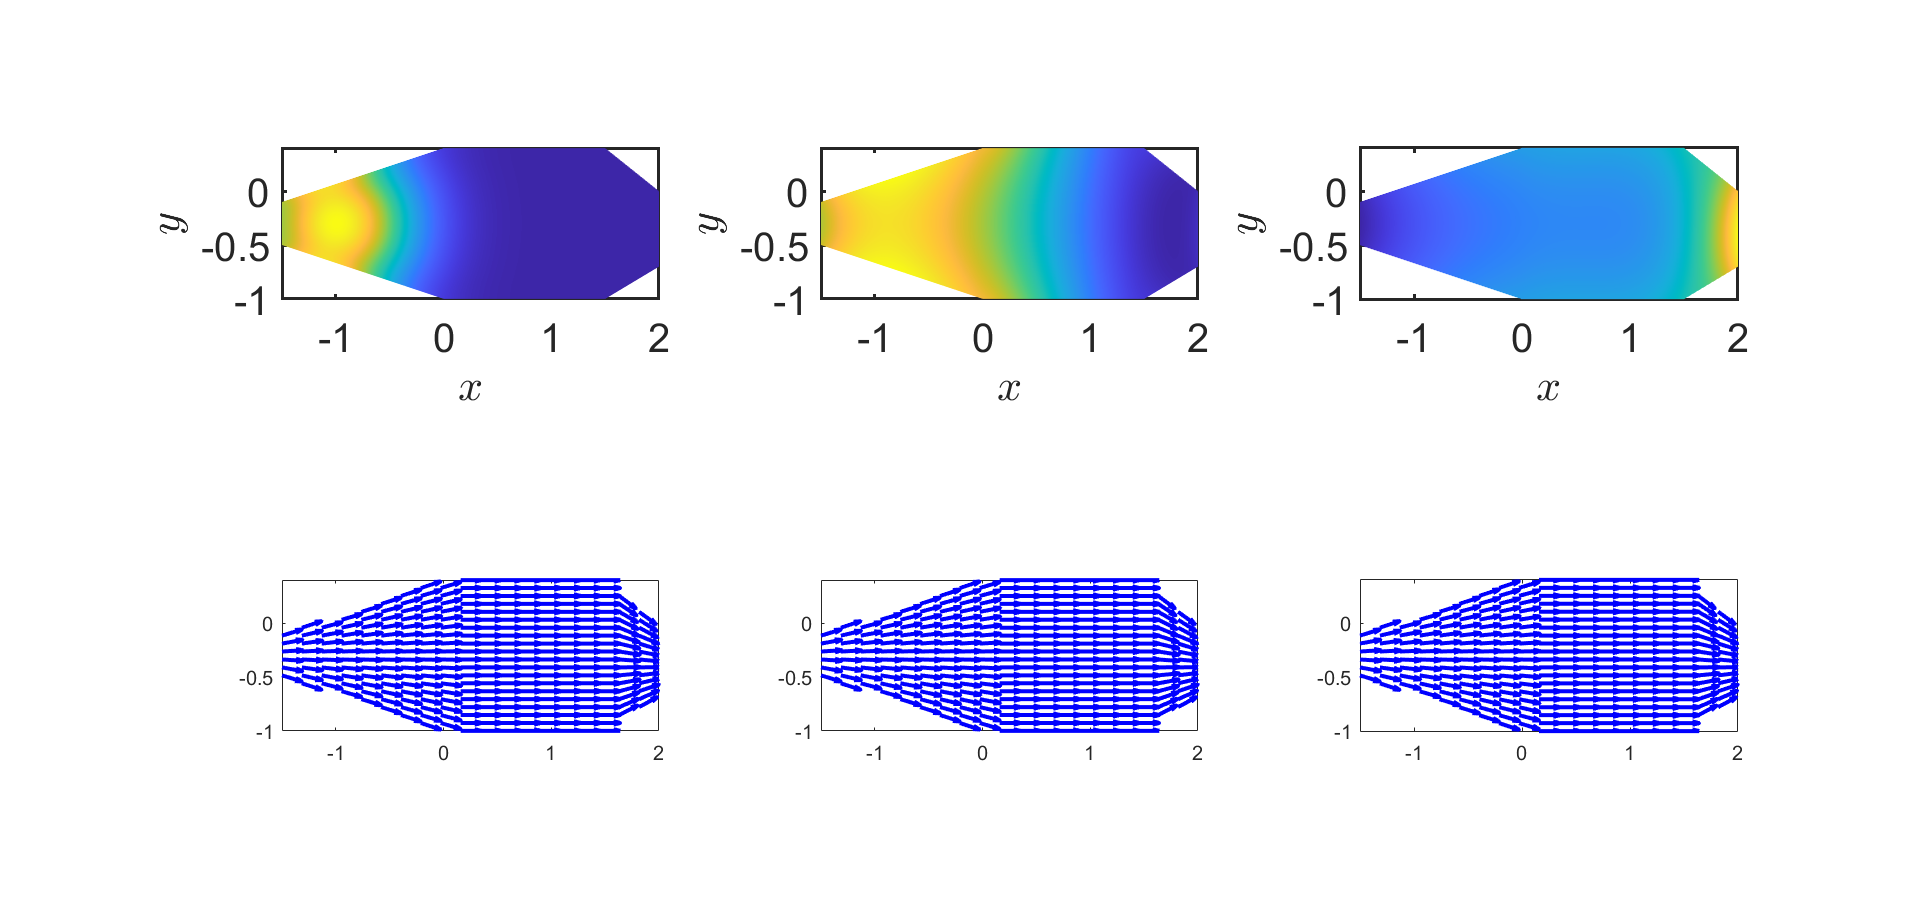
\includegraphics[scale=0.3]{FW31.png}
	\caption{Example 3, $\widehat \rho$, $\kappa = 1$} 
	\label{FEx3c}
\end{figure}
\begin{figure}[h]
	\centering
	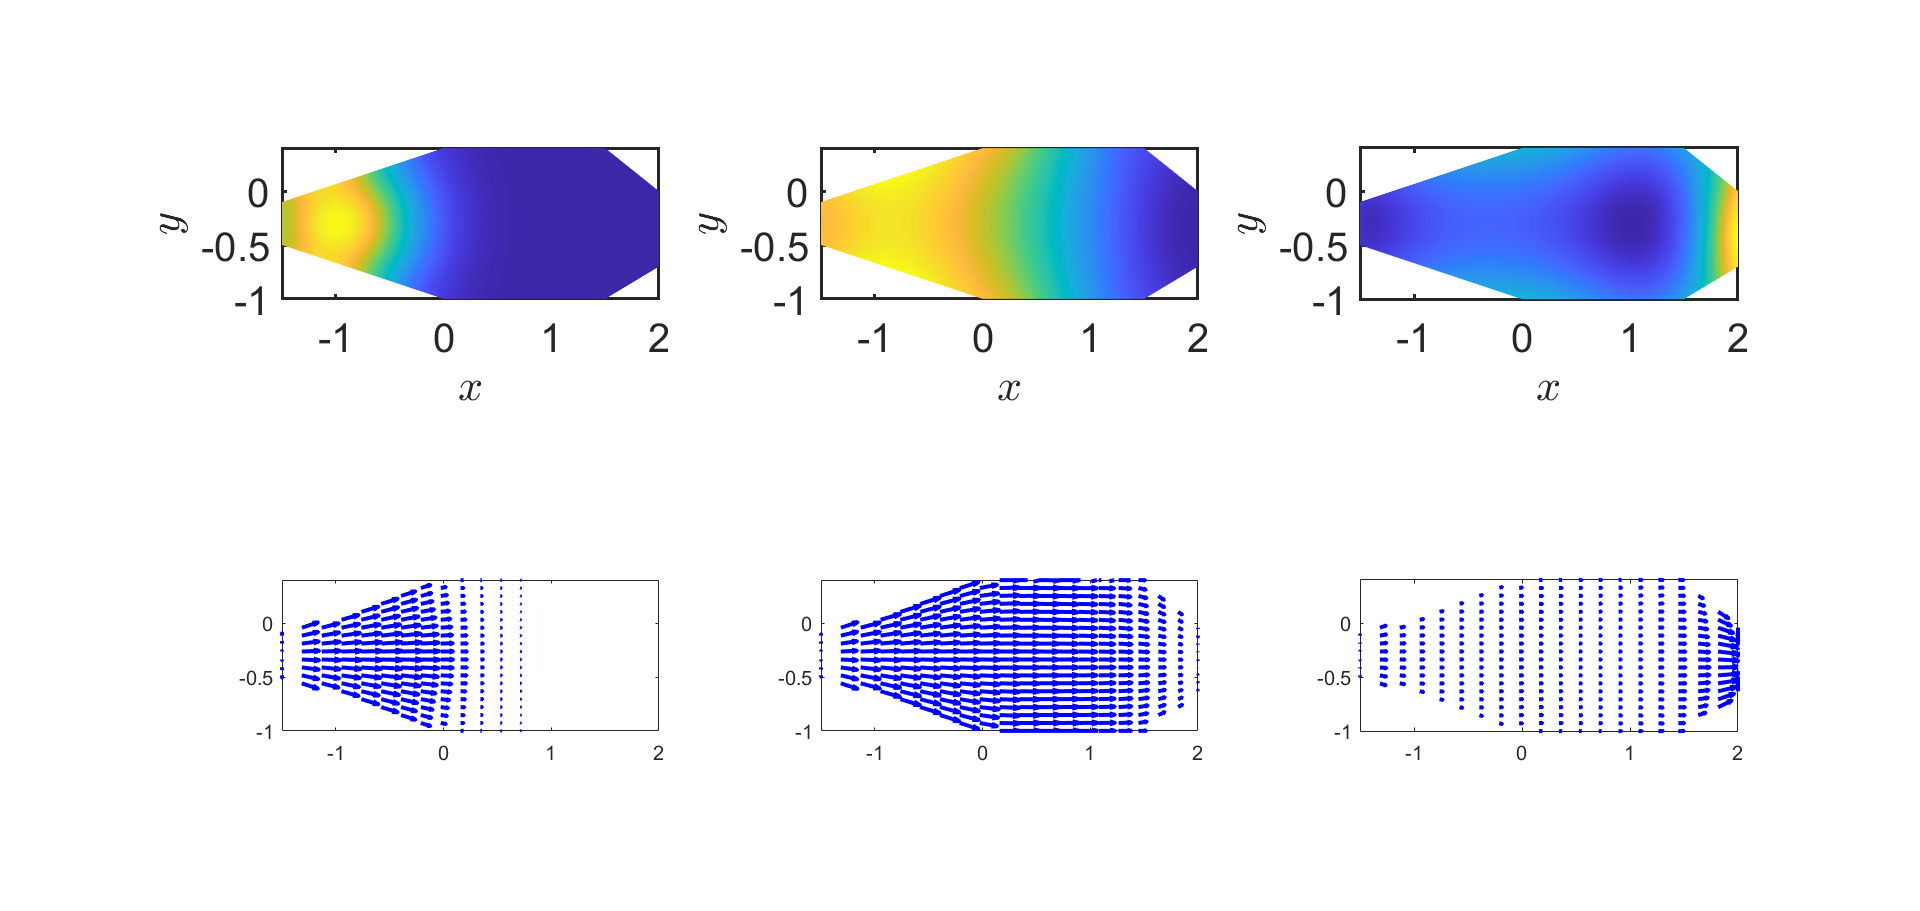
\includegraphics[scale=0.3]{Opt31.png}
	\caption{Example 3, optimal $\rho$ and $\w$, $\kappa = 1$} 
	\label{FEx3d}
\end{figure}	
	
	
\end{document}